\documentclass[conference]{IEEEtran}
\usepackage{latexsym}
\usepackage{epsf}
\usepackage{epsfig}
%\usepackage{a4wide}
\usepackage{amssymb}
\usepackage{graphicx}
\usepackage{multirow}
\usepackage{float}
%\usepackage{enumitem}
%\usepackage{enumerate}
%\usepackage[options]{natbib}
\usepackage{verbatim} 
\usepackage{slashbox}
\usepackage{subfig}
\usepackage{float}
\usepackage{cite}
\usepackage{url}
%\usepackage{algorithmic}
%\usepackage{algorithm}
\usepackage[super]{nth}
\setlength{\textfloatsep}{5pt}

\hyphenation{op-tical net-works semi-conduc-tor IEEEtran}
\begin{document}
% paper title
\title{Level-crossing analog-to-digital converter for high frequency content signals}
\author{\IEEEauthorblockN{Janamani C. Ayyangalam and A. N. Chandorkar}
\IEEEauthorblockA{Department of Electrical Engineering,\\
Indian Institute of Technology-Bombay, Mumbai, India.\\
Email: janamani@ee.iitb.ac.in, anc@ee.iitb.ac.in}}
% make the title area
\maketitle
\begin{abstract}
	This paper presents a Level-Crossing Analog-to-Digital Converter (\mbox{LC-ADC}) architecture which improves the performance compared with conventional \mbox{LC-ADC's} by using successive approximation kind of method. Advantages of the proposed \mbox{LC-ADC} over conventional \mbox{LC-ADC's} are less conversion time, when the input analog signal varies rapidly and reduced loop delay, which is achieved by incorporating priority encoder in place of Up-Down counter in conventional \mbox{LC-ADC's}.   
\end{abstract}

% no keywords
\IEEEpeerreviewmaketitle






\section{Introduction}	
	In applications like bio-medical signals, temperature sensors, pressure sensors, speech signals and ultrasound signals, continuous observation of analog input signal is necessary. Conventionally for converting these analog signals into digital signals Nyquist \mbox{ADC's} are used. However, these signals are constant for most of the time, with brief high frequency content. This leads to oversampling for most of the time, leading to more power consumption without yielding new information~\cite{akopyan2006level}.\par

	
	\mbox{LC-ADC's} are best suited for signals which have occasional high frequency content, but are constant for most of the time~\cite{trakimas20080}~\cite{kozmin2009level}. \mbox{LC-ADC's} generates new information only when the analog input crosses one of the quantization levels. This leads to low activity in the circuit most of the time. This makes the \mbox{LC-ADC's} more power efficient compared to Nyquist ADC's and reduces unnecessary samples.\par


	Most of the reported \mbox{LC-ADC's} suffer from the large loop delay which results in slope overloading error~\cite{trakimas2011adaptive}~\cite{agarwal2009adaptive}. The authors of~\cite{kurchuk2009signal} have suggested signal dependent variable resolution quantization technique to reduce slope overload error. This technique uses a slope detector at the input to measure the slope of the input signal. Depending on the slope of the input signal it changes the resolution of the \mbox{LC-ADC}. The effectiveness of this technique depends on how accurately the slope is measured by the input slope detector. In this technique the complexity of the \mbox{LC-ADC} increases with the number of bits to represent the slope.\par


	The authors of~\cite{agarwal2009adaptive} have suggested variable input slope dependent technique to reduce slope overload error. In this technique previous bits are stored, based on which the slope is estimated and the resolution of \mbox{LC-ADC} is adjusted. This technique has significant chances of misinterpreting the output when the slope of the input signal is changing. Apart from misinterpretation, the complexity of the circuit is proportional to the number of bits used to set its resolution. \par


	The architecture proposed in this paper solves slope overloading error problem with minimal increase in complexity. The proposed technique is purely deterministic. In addition to improved performance, the proposed architecture can be reconfigured to operate in Nyquist mode. The proposed architecture also reduces power consumption when operated in Nyquist mode as compared to conventional successive approximation \mbox{ADC's}.\par


	Rest of this paper is organized as follows. Section II discusses the background theory of level-cross sampling scheme. Section III describes the Level-Crossing ADC architecture. Section IV describes the proposed ADC architecture. Simulation results of the proposed ADC architecture are presented in Section V and Section VI concludes the paper.\par







\section{Background Theory}
	 
	Level-cross sampling scheme is the dual of the Nyquist sampling scheme. In Nyquist \mbox{ADC's} the samples are taken at fixed intervals of time with reference to the clock signal. The minimum clock signal is chosen to be twice the maximum frequency of the analog input signal. For signals in which the frequency content is very low for most of the time, with rare occurrences of high frequency contents, it leads to over sampling. Hence, taking samples at regular intervals of time unnecessarily increases circuit activity, which in turn increases the power consumption~\cite{sayiner1996level}.\par

	\mbox{LC-ADC's} are driven by the level-crossing rather than by clock ie., the conversion process triggers when the analog input crosses any of the quantization levels, these are best suited for asynchronous and low power applications~\cite{allier2003new}. The level-cross sampling scheme can be understood by using Fig.~\ref{fig:ECG}, which shows a typical ECG signal~\cite{}. The dotted lines represent quantization levels. \par

\begin{figure}[ht]
	\begin{center}
		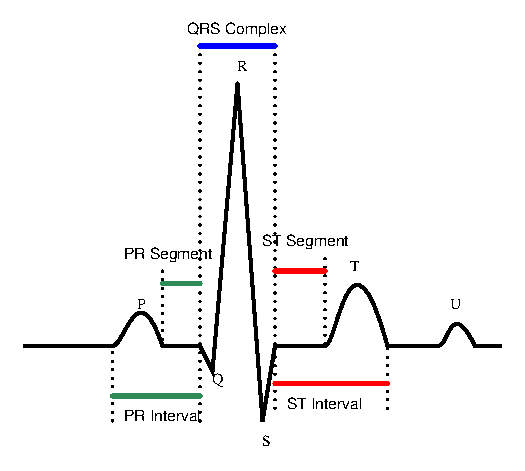
\includegraphics[height=8.5 cm, angle=270]{./Figures/ECG.ps}
		\caption{level-cross sampling scheme for an ECG signal}
		\label{fig:ECG}
	\end{center}
\end{figure}

	In \mbox{LC-ADC's}, for an N-bit hardware resolution, $2^{N}-1$ quantization levels are regularly spaced along the amplitude range of the analog input signal. A sample is taken only when the analog input signal crosses any one of the $2^{N}-1$ quantization levels. The shape of the analog input signal can be preserved by calculating the time difference between two successive samples. Thus, outputs from \mbox{LC-ADC's} are amplitude and time data pairs, unlike that of Nyquist \mbox{ADC's} where the output consists of only amplitude data. Table.~\ref{tab:DNL} shows the difference between Nyquist and Level-Crossing sampling schemes. \par



\begin{table}[t]
	\caption{Difference Between Nyquist \& Level-Crossing sampling schemes}
	\label{tab:DNL}
	\begin{center}
	\resizebox{8.5cm}{!}{
		\begin{tabular}{c|c|c|}
			\cline {2-3} %\hline
		 	&{Nyquist Sampling} & {Level Cross Sampling} \\ \hline
			\multicolumn {1}{|c|} {Conversion Trigger} &   {Clock} &  {Level Crossing} \\ \hline
			\multicolumn {1}{|c|} {Amplitude} &  {Quantized} &  {Exact Value} \\ \hline
			\multicolumn {1}{|c|} {Time} &  {Exact Value} &  {Quantized} \\ \hline
			\multicolumn {1}{|c|} {SNR Dependency} &  {Number of Bits} &  {Timer Period} \\ \hline
			\multicolumn {1}{|c|} {Converter Output} &  {Amplitude} &  {Amplitude \& Time} \\ \hline
		\end{tabular} }	
	\end{center}
\end{table}

	The time taken from analog input crossing one of the quantization levels to complete conversion is called loop delay. The loop delay of the LC-ADC decides the maximum input signal frequency which can be tracked without slope overload error by the ADC. The proposed architecture is aimed to reduce this loop delay so that it can track high frequency components in input analog signal without slope overloading error.\par



\section{LC-ADC Architecture}

	The block diagram of the \mbox{LC-ADC} is shown in Fig.~\ref{fig:LCADC}. Depending on the difference between amplitudes of $V_{ref}$ and $V_{inp}$, the difference quantificator sets the value of $INC$ and $DCR$. Where $V_{ref}$ is the analog signal corresponding to the present contents of the up-down counter and $V_{inp}$ is analog input signal. If the difference between $V_{ref}$ and $V_{inp}$ is less than \mbox{$V_{LSB}/2$}, both $INC$ and $DCR$ signals will be low, where $V_{LSB}$ is the hardware resolution of the LC-ADC. If the difference between $V_{ref}$ and $V_{inp}$ is more than \mbox{$V_{LSB}/2$}, then depending on the direction of analog input signal one of the signals $INC$ or $DCR$ will be set. Table.~\ref{tb:ODQ} shows the values set by the difference quantifictor. \par

\begin{figure}[ht]
	\begin{center}
		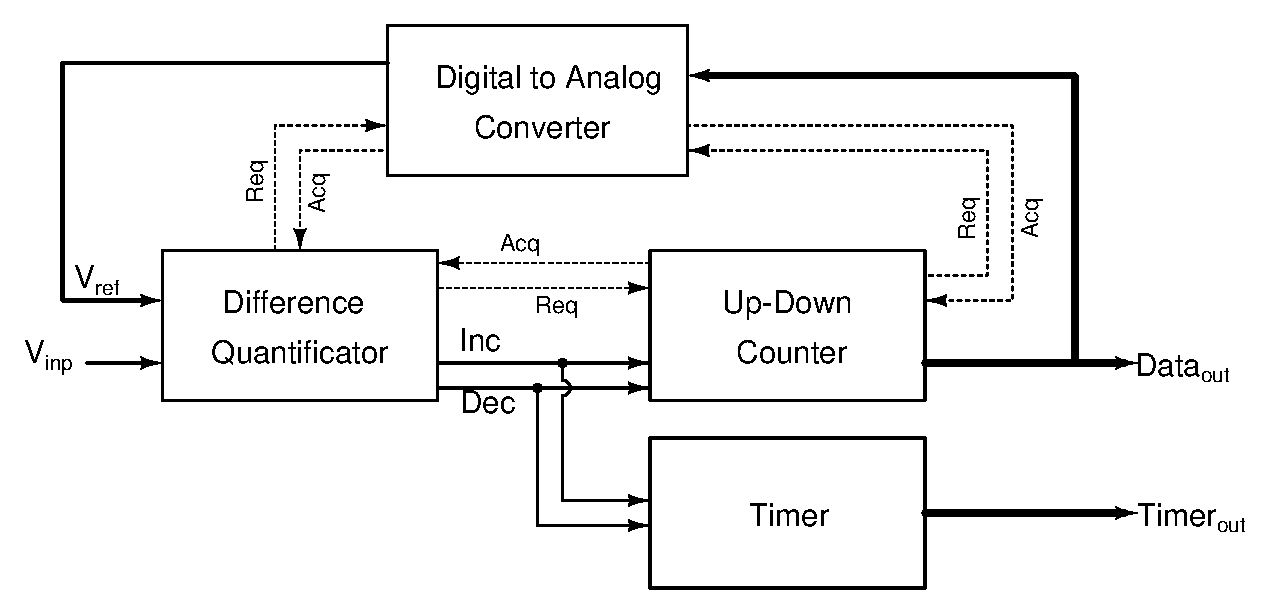
\includegraphics[width=8.5 cm, angle=360]{./Figures/LCADC.ps}
		\caption{Asynchronous Level-Crossing ADC~\cite{allier2005120nm}}
		\label{fig:LCADC}
	\end{center}
\end{figure}

\begin{table}[t]		
	\begin{center}
	\caption{Operation of differnce quatificator}
	\label{tb:ODQ}
		\begin{tabular}{| c | c | c | c |}\hline
	 		Condition & $INC$ & $DCR$ & $Up-down Counter$  \\ \hline
			\multicolumn {1}{|c|} { $V_{ref}$ - $V_{inp}$ $<$ $|V_{LSB}/2|$ } & $Low$  & $Low$ & Nothing  \\ \hline
			\multicolumn {1}{|c|} { $V_{ref}$ + $|V_{LSB}/2|$ $<$ $V_{inp}$ } & $High$  & $Low$ & Increment  \\ \hline
			\multicolumn {1}{|c|} { $V_{inp}$ + $|V_{LSB}/2|$ $<$ $V_{ref}$ } & $Low$ & $High$ & Decrement \\ \hline
		\end{tabular}
	\end{center}
\end{table}

	There will be no activity in the up-down counter if both outputs of the difference quantificator are $Low$. If any one of the difference quantificator output $INC$ or $DCR$ is $High$, then these outputs trigger the up-down counter. Depending on which output of the difference quantificator is $High$, contents of up-down counter increments or decrements. The outputs of the difference quantificator also triggers timer block, which is used to track the elapsed time between previous and present samples. \par

	The outputs of the LC-ADC are contents of up-down counter and Timer data pairs, the output of the up-down counter is fed to the digital-to-analog converter (DAC) which converts the present value in the up-down counter to it's corresponding analog value, which refers to the present analog value for further comparison with the analog input signal in difference quantificator to find out whether the input signal is increasing or decreasing. \par

	Generally the up-down counter in LC-ADC is implemented using an adder-subtractor circuit. As the number of bits in up-down counter increases the delay in calculating the up-down counter value increases when a trigger generated by the difference quantificator. This increase in delay results in increased loop delay of the LC-ADC. If the loop delay of the LC-ADC increases, it effectively reduces the maximum frequencies in the analog input signal which it can track without slope overload error will be decreased. \par

	 As up-down counter uses an adder-subtractor circuit, which increases or decreases the contents of the up-down counter linearly. If the analog input changes rapidly, for example ``0010" to ``1001" in a 4-bit hardware resolution LC-ADC, then it requires 7 clock cycles to track that value. Fig.~\ref{fig:SOE} shows the slope overload error problem. The maximum frequency of the input with which the LC-ADC can track without slope overload error can be calculated by using loop delay of the LC-ADC~\cite{allier2005120nm}. \par

\begin{figure}[ht]
	\begin{center}
		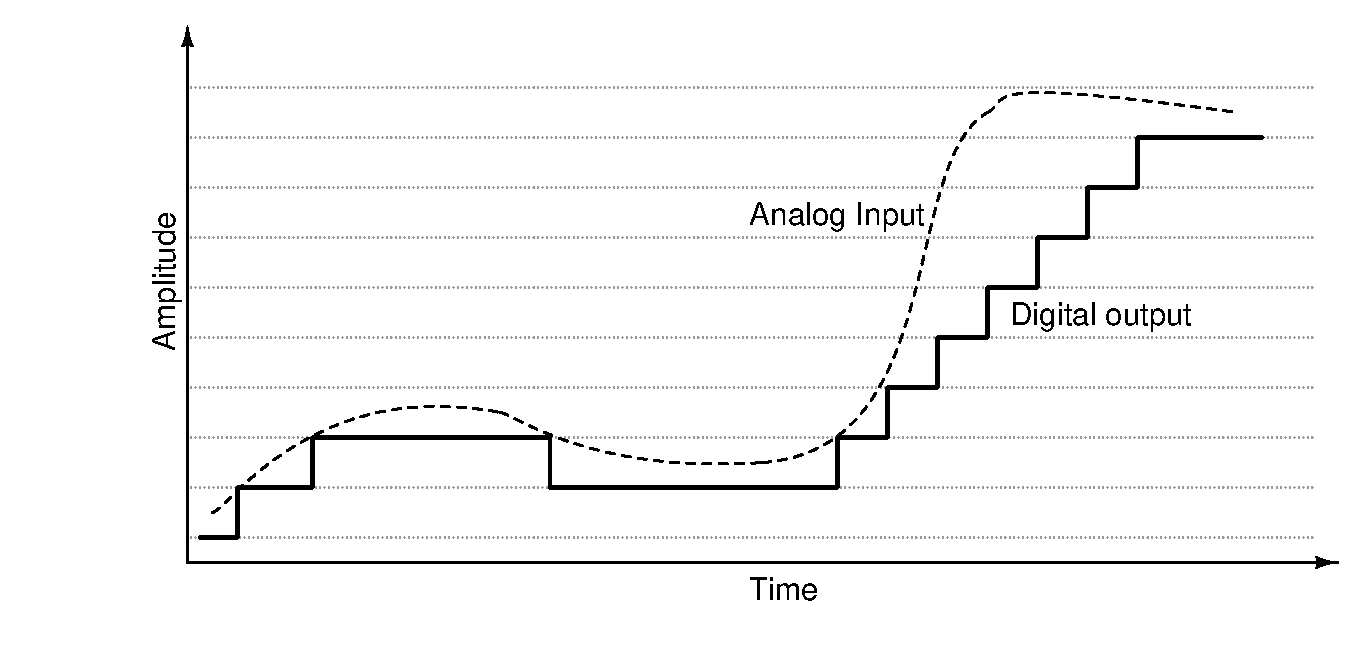
\includegraphics[width=8.5 cm, angle=360]{./Figures/SOE.ps}
		\caption{Slope overloading error in LC-ADC}
		\label{fig:SOE}
	\end{center}
\end{figure}


\section{Proposed Architecture}

	The proposed architecutre is desigened in such a way that the loop delay is reduced by changing up-down counter with a more intilligent controller circuit when the analog input changes rapidly. Which tracks the analog input in more intilligent manner. The operation of Contrroller is shown in Fig.~\ref{fig:FLOWCHART} as a flow chart for 8-bit hardwear resolution. \par

	The proposed controller tracks the analog input in logarathmic fashion rather then linear fshion which is generally followed in conventional LC-ADC's. At maximum the proposed LC-ADC takes $2N$ clock cycles for complete the process if the analog input changes from minimum to maximum, where as the conventional LC-ADC's which use up-down counter will take $2^N$ clock cycles to complete the operation when the analog input changes from minimum to maximum value.\par

\begin{figure}[ht]
	\begin{center}
		\includegraphics[width=8.5 cm, angle=360]{./Figures/FLOWCHART.ps}
		\caption{Operatoion of controller circuit as a Flow Chart}
		\label{fig:FLOWCHART}
	\end{center}
\end{figure}

	The controller works as follows, when a trigger signal genreted by the difference quantificator, the controller checks for which signal it is, If it is a $INC$ signal then it chcks for a '0' from LSB to MSB, if it finds a 0 at LSB then changes LSB from 0 to 1, it effectively implies as increasing the present data by 1. If it does find 0 in LSB, it checks next bit to LSB, untill it finds a 0. Then it changes the 0 into 1 and applies to the capacitor array to fix the as in conventional SAR ADC's. It uses the same DAC which is used to generate the reference signal for difference quantificator.\par

	The intialization process ends when the refence signal $V_{ref}$ is greater then $V_{inp}$ at this point of time the bits from current position to LSB all will be set to '1'. Then the bits from LSB to 1-bit less to current postion will be set to '0' and normal succsive aprroximation algoritham is implemented to set or rest the bits. This procedure effectively checks untill which bits if we make so that the analog input will be less then refernce voltage when minimum bits sets. Then it checks for the correct value. \par

	In case of $DCR$ signal is generated by differnce quantificator, then the cotroller circuit for '1' from LSB to MSB, if it finds a '1' at LSB, then it changes the '1' into '0', it effectively implies as decreasing the present data biy '0'. If it is does not find '1' in LSB then checks for the next bit to LSB untill it finds a '1'. Then the controller changes the '1' into '0' and applies to the cappacitor array to fix the as in conventional SAR ADC. \par

	The intialization process ends when the reference signal $V_{ref}$ less then analog input signal $V_{inp}$ at this point of time all bits from LSB to prsent bit are '0'. the present bit should be '1' and normal succsive approximation algoritham is implimented to set or reset the bits. This procdure is effectively checks untill which bits if we make so that the analog input will be greater then the refence voltage when all bits are reset from LSB to present bit. Then it checks for the correct value. The controller circuit is designed in such a way that when the trigger intiates the operation, then the effects of $INC$ or $DCR$ signals will be elimimated untill the operation is completed.  \par


	Fig. 






%	The flowchart in Fig.XYZ shows the working of the proposed ADC architecture. In conventional SAR ADC's MSB is set, which takes the DAC output  to $V_{ref}/2$. If the input is higher than $V_{ref}/2$, the MSB is left set otherwise it is reset. Then the next MSB is evaluated in the same way. This procedure is repeated for all the subsequent bits. This approach takes $N$ clock cycles for an N-bit ADC.\par 


%	In the proposed approach the difference quantificator gives the relative position of the analog input with respect to the previous quantized value. If the $INC$ is $HIGH$, then the value of analog input is higher then the previous quantized value. In conventional search when the input is less than the quantized value for the 1$^{\textnormal{st}}$ time, the $i^{\textnormal{th}}$ bit which was being tested is reset. All $(i-1)$ bits from the MSB are set at this point. In the proposed architecture since $INC$ gives us the information that the analog input is higher then the previous quantized value. These $(i-1)$ bits are inherited from the previous output. \par


%	Similarly, in the other case when $DCR$ is $HIGH$, the first $(i-1)$ zeros are inherited from the previous output. Fig.~\ref{fig:Section33} illustrates the difference in the search sequence between conventional SAR and proposed ADC architecture. Following example demonstrate the situation for the proposed ADC which leads to reduction in activity of conversion circuit. \par


%	Example 1: When analog input is increasing if the contents of successive approximation register are ``11010110'', then the value assigned to Shift Register is ``00100000'' and the value assigned to successive approximation register is ``11000000'', which results in reduction of two clock cycles.\par

\begin{table}[h]		
	\begin{center}	
		\begin{tabular}{ c  c  c  c  c  c  c  c  c }
			Shift Reg  & 0 & 0 & \textbf{1} & 0 & 0 & 0 & 0 & 0 \\
				   &  &  & $\Uparrow$ & & & & & \\		
	 		\textbf{Output}   & \textbf{1} & \textbf{1} & \textbf{0} & X & X & X & X & X \\
				   & $\Downarrow$ & $\Downarrow$ & & & & & & \\
			SA Reg     & \textbf{1} & \textbf{1} & 0 & 0 & 0 & 0 & 0 & 0 \\			
		\end{tabular}
	\end{center}
\end{table}


%	Example 2: When analog input is decreasing if the contents of successive approximation register are ``00001110'', then the value assigned to Shift Register is ``00001000'' and the value assigned to successive approximation register is ``00000000'', which results in reduction of four clock cycles.\par

\begin{table}[h]
\begin{center}	
		\begin{tabular}{ c  c  c  c  c  c  c  c  c }
			Shift Reg  & 0 & 0 & 0 & 0 & \textbf{1} & 0 & 0 & 0 \\
				   & &  &  &  &$\Uparrow$ & & & \\	
	 		 \textbf{Output}   & \textbf{0} & \textbf{0} & \textbf{0} & \textbf{0} & \textbf{1} & 1 & 1 & 0 \\
				   & $\Downarrow$ & $\Downarrow$ &  $\Downarrow$ &  $\Downarrow$ & & & & \\
			SA Reg     & \textbf{0} & \textbf{0} & \textbf{0} & \textbf{0} & 0 & 0 & 0 & 0 \\
			
		\end{tabular}
	\end{center}
\end{table}




\section{Simulation Results}

	The proposed ADC has been simulated with UMC 180nm Mixed-Mode CMOS technology. Figure XXX shows the layout of the proposed ADC. Figure XXX shows INL and DNL plots. Table.~\ref{tb:COTD} shows the summary of post layout simulation results. The simulation result of the ADC is shown in Figure XXX for an ECG signal. 



\section{Conclusion}
	In this paper, we presented a power efficient ADC which can track high speed analog input signals, using UMC 180nm CMOS technology. Simulation results show that the total power consumption is below XXX at 1.8V and Figure of Merit(FoM) is XXX. This ADC can be effective in applications like ECG, speech processing, some of ultrasound applications, pressure and temperature controllers where signal vary during a small period of time and quiet most of the time. \par



\section*{Acknowledgement}
The authors would like to thank Department of Information Technology, Government of India, for sponsoring Ph.D through SMDP-II, VLSI and MHRD project (05-DL-001).

\bibliographystyle{IEEE}
\bibliography{ISICRef}

\end{document}

